\chapter{Beam Position Monitor Requirements}
\section{Beam size monitoring Compatibility}
The Beam Size Monitor (IPBSM) measures the scattered photons from an electron-photon collission between the particle bunch and a perpendicular interference pattern generated by high intensity laser perpendicular to the bunch trajectory \cite{Shintake1992453}. Fig. (\ref{f:IPBSM}) shows an schematic design of the IPBSM.
\begin{figure}[htb]
 \begin{center}
  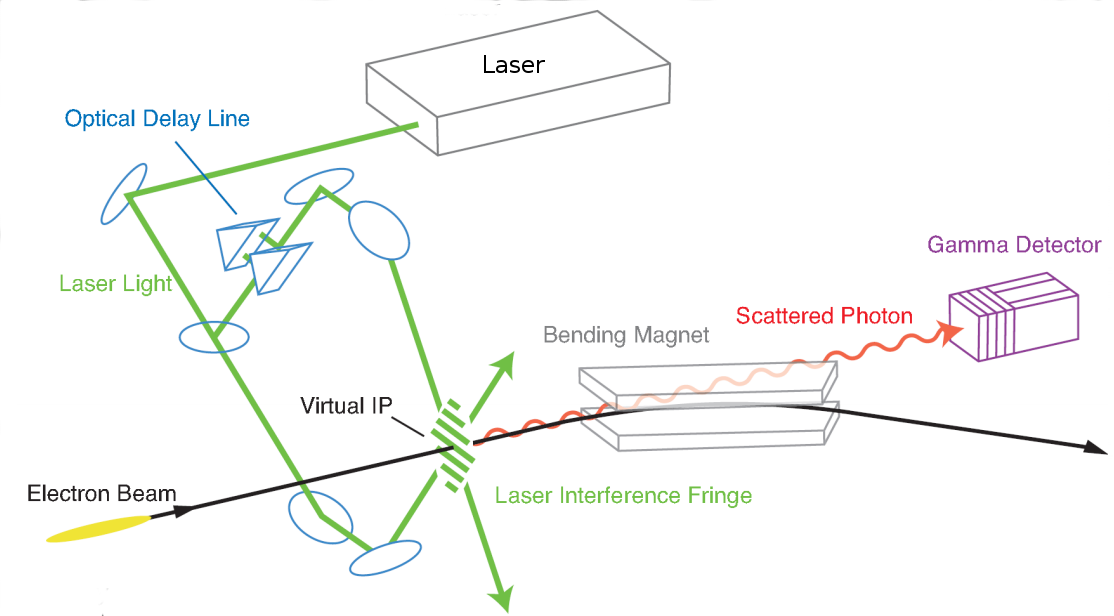
\includegraphics[angle=0,scale=0.5]{IPBSM_1.png}\caption{IPBSM schematic design. The particle beams crosses the interference pattern generated by a perpendicular beam. The number of electron-photon interactions varies with the fringe size and the particle beam size.}\label{f:IPBSM}
 \end{center}
\end{figure}
The current IPBSM at ATF2 \cite{Jackelinethese} is installed in a vertical optical table where the laser incident angle can be adjusted to change the interference fringe size giving four orders of magnitude of beam size resolution. Fig. (\ref{f:IPBSMangles}) shows the beam path along the vertical optical table for three angles modes and the correspoding range of beam measurements.\par
\begin{figure}[htb]
 \begin{center}
  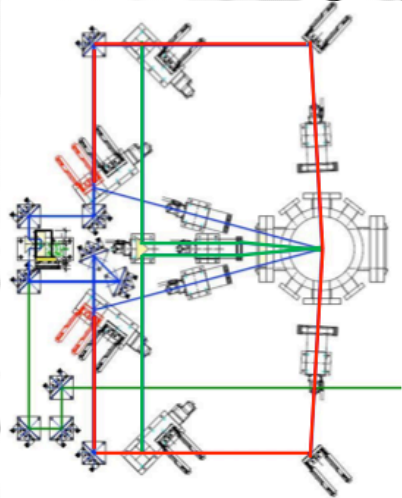
\includegraphics[angle=0,scale=0.35]{IPBSM_angles.png}
  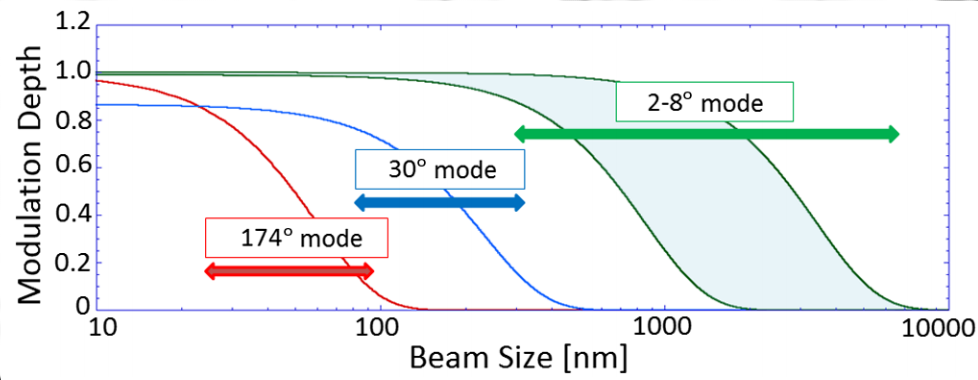
\includegraphics[angle=0,scale=0.455]{IPBSMreso.png}
  \caption{IPBSM laser path and beam size resolution for the angle modes : $2\sim8$\degree in green, 30\degree in blue and 174\degree in red.}\label{f:IPBSMangles}
 \end{center}
\end{figure}
The beam positioning system should not interfere with the IPBSM measurements. Therefore, mechanical dimensions and weight should be restricted to those supported by the vertical optical table. This will allow to have a common reference point between the two structures.\par 
In addition, the longitudinal direction must be set to match the lattice IP position, the IPBSM IP and the beam position monitor in a common region. A tolerance of several cm could be of great advantage due to the dimensions and apertures of the optical components in the laser path.\par
Synchronization between the beam position monitor data and the IPBSM data would allow to mitigate the effect of large beam fluctuations on beam size measurement by discarding trajectories too far from the IPBSM best resolution spot.\par
\section{Optics in the IP Region}
The $\beta^*$ functions at the IP can be set by changing the upstream magnets strength. Three configurations are normally used : 1BX1BY, 10BX1BY, and 100BX1000BY, where the factor indicates the number of times that the original $\beta^*$ has been amplified.\par
The 1BX1BY optics has the original design parameters. Here the angular divergence of the beam is $0.35$mrad vertically and $0.52$mrad horizontally in the IP region. \par
The 10BX1BY preserves the $\beta_y^*$ goal while relaxing the tolerance to multipole errors in magnets by increasing ten times the original $\beta_x^*$, making them comparable with those of ILC 500GeV \cite{PhysRevSTAB.17.023501}. This optics has been plot in Fig. (\ref{f:FF_MADX}) and it is currently used in operation.\par
The 100BX1000BY optics sets a parallel beam through the IP area, principally used to avoid the issues of large angle divergence displayed by the 1BX1BY optics.\par
Even smaller $\beta_y^*$ functions have been explored recently at ATF2 aiming to estimate lower $\beta^*$ tunability and IPBSM limitations \cite{PateckiLowBeta}.\par
Figure (\ref{f:BXYoptics}) shows the beam size in vertical and horizontal plane for several optics combinations in a region of several cm around the IP. It also shows clearly how the beam divergence affects the beam size along the IP region. Now, considering the measurement of beam position, it has been shown by previous measurement results that beam jitter upstream the FD is around 10$\sim$20\% of beam size on the vertical plane and 5$\sim$10\% on the horizontal plane \cite{PateckiJitter}. 
\begin{figure}[htb]
 \begin{center}
 \hspace*{-1cm}
 \begin{subfigure}[b]{0.45\textwidth}
  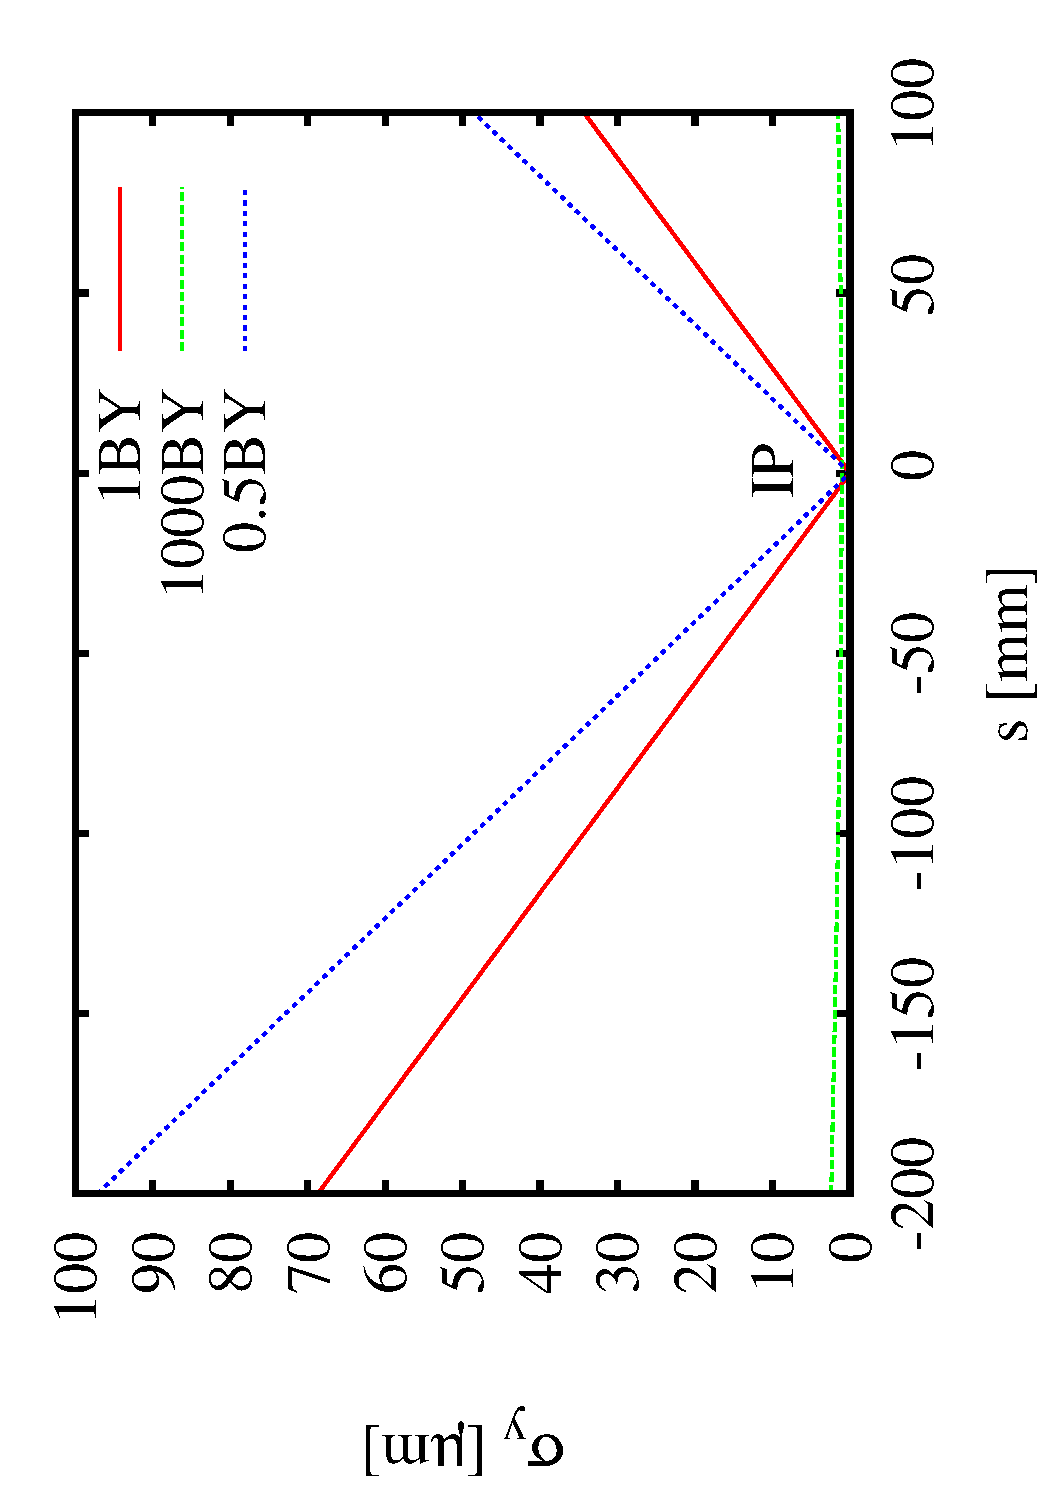
\includegraphics[angle=-90,scale=0.32]{optics_requ.pdf}\caption{Vertical beam size near the IP.}\label{f:opticsBY}
 \end{subfigure}\hspace{0.5cm}
\begin{subfigure}[b]{0.45\textwidth}
  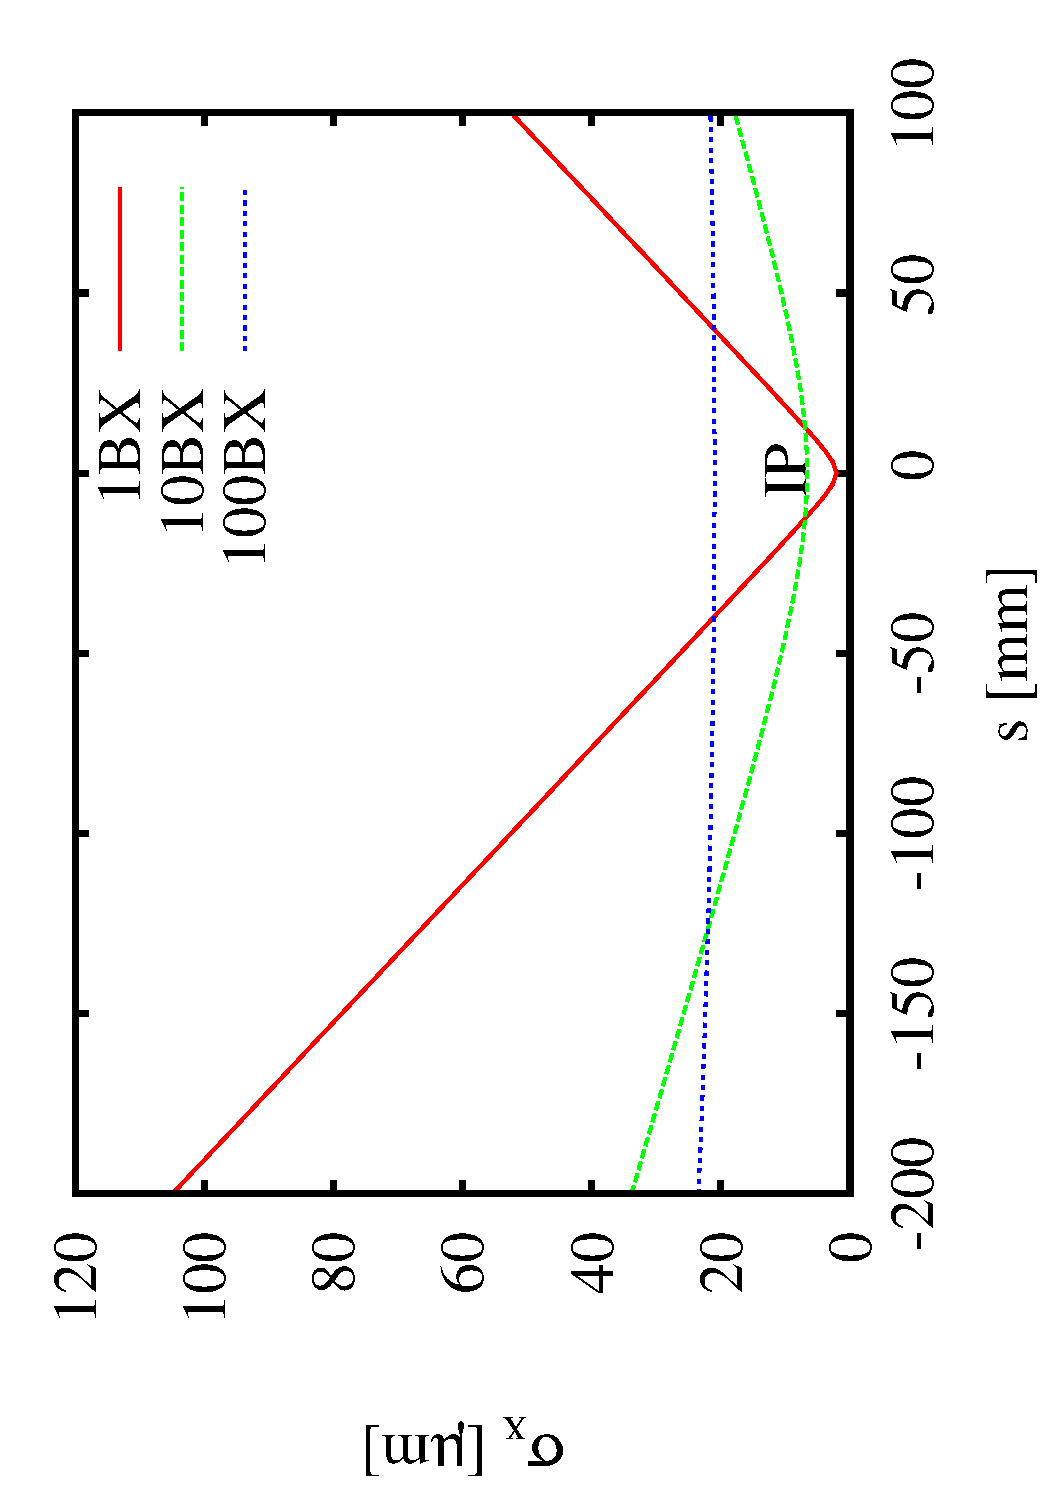
\includegraphics[angle=-90,scale=0.32]{optics_BX.pdf}\caption{Horizontal beam size near the IP.}\label{f:opticsBX}
 \end{subfigure}
  \caption{Vertical and horizontal beam sizes for 1BY, 1000BY, and 0.5BY in the vertical plane, and 1BX, 10BX and 100BX in the horizontal plane.}\label{f:BXYoptics}
 \end{center}
\end{figure}
If the jitter to beam size proportion is preserved in the FD and IP region, then, a minimum dynamic range between $5\sim10\mu$m is required for vertical position measurement with the previously mentioned optics and 10\% jitter. While the horizontal plane dynamic range must be close to $10\mu$m.\par
Having in mind the stabilization of the beam trajectory at the IP by few nanometers, it is clear that beam monitoring system must have a resolution equal or better than this. This implyes the big requirement of $10^{-4}$ resolution, linearity and stability over the entire dynamic range.\par
Knowing the beam trajectory with this precision is valuable information for beam tuning that could bring the beam jitter down, relaxing the dynamic range/resolution requirements, including the identification of local jitter sources in the FD and IP region.\par
\section{Feedback}
Under the goal 2 scope, the beam stabilization must be operative in different configurations : intra-train targeting pulse to pulse measurement and correction, inter-train stabilization targeting the train to train measurement and correction, both relying in the correlation measurement and correction in several scales of time.\par
Probably the most direct type is an intra-train active stabilization by feedback in the IP region. It consist in the measurement of a first bunch trajectory to correct the second and following. This avoids the propagation to upstream correctors and reduces the time latency restriction for the processing electronics determined by the time between pulses at maximum.\par
The ILC and CLIC colliders differ largely in this parameter : 0.5ns for CLIC and 367ns for ILC. The minimum bunch spacing at ATF is 2.8ns \cite{ATF2prop,BurrowsIntraTrain}, therefore it can not test CLIC specifications. However, in single-bunch mode, a maximum of three bunches with 154ns spacing are stored in the damping ring and can be used to test the intra-train feedback conceived by FONT \cite{BurrowsIntraTrain2,BurrowsIntraTrain3}.\par
The beam position monitor response and processing electronics latency must remain inside the tolerable values to perform feedback between two bunches.\par
